\documentclass[fleqn,10pt,lineno]{manuscript}
%%\usepackage{setspace}
%%\doublespacing
\usepackage{soul}
\usepackage[utf8]{inputenc}

\newcommand{\beginsupplement}{%
        \setcounter{table}{0}
        \renewcommand{\thetable}{S\arabic{table}}%
        \setcounter{figure}{0}
        \renewcommand{\thefigure}{S\arabic{figure}}%
     }

\title{A Structural and Functional Bioinformatics Study of QTY-designed Retinylidene Proteins}

\author[1]{Siqi Pan}
\author[2]{Shuguang Zhang}
\affil[1]{Shanghai World Foreign Language Academy, 400 Baihua Street, Shanghai 200233, China}
\affil[2]{Lab of Molecular Architecture, Media Lab, Massachusetts Institute of Technology, 77 Massachusetts Avenue, Cambridge, MA 02139, USA}

\corrauthor[2]{Shuguang Zhang}{Shuguang@MIT.EDU}

\keywords{Keyword1; Keyword2; Keyword3}
\begin{abstract}

Abstract of paper -- leave until everything is written. 

\end{abstract}

\begin{document}

\flushbottom
\maketitle
\thispagestyle{empty}

\section*{Introduction}

Intro

* Families of opsins - vertebrate vs. bacterial

* General features of vertebrate opsin; structure and function

* Activation mechanism of rhodopsin

* Expression, function of each opsin

* General features of bacterial opsin; structure, function, applications

* Why solubilize

* History of solubilizing studies of rhodopsin and bacteriorhodopsin

* Existing QTY studies

* Intro to AlphaFold

* Intro to GROMACS

* Existing rhodopsin bioinformatics studies


\section*{Results and Discussion}

Results

* discuss the QTY code

* describe and explain Table1

* describe and explain Fig1

* describe and explain Fig2
	- I need more discussion here

* describe and explain Fig3

* discuss AlphaFold3 predictions

* describe, explain, discuss MD results (Fig3 and Fig4)
	- I need more discussion here

* future scopes and potential applications

* conclusion

\section*{Methods}

Methods

* protein sequences UniProt

* AlphaFold3 server

* superimposition (PDB, AlphaFold, PyMOL)

* Structure visualization (PyMOL, ChimeraX)

* MD simulation (GROMACS, etc.; detailed params; analysis techniques)


\section*{Supplementary Material}

The supplementary material can be found at...


\section*{Data Availability Statement} 

The data for ... can be found at...


\section*{Author contributions}

Detailed author contributions


\section*{Financial Support}

No funding was received for this project. 


\section*{Acknowledgments}

Thanks to ... for ...


\section*{Competing Interests}

The authors declare no conflict of interest.


\section*{Ethics Statement}

There are no ethics issues related to the research in this paper. No animal or human data...


\bibliography{references}

\begin{table}[h]
	\centering
	\caption{Protein characteristics}
	\label{tb:characteristics}
	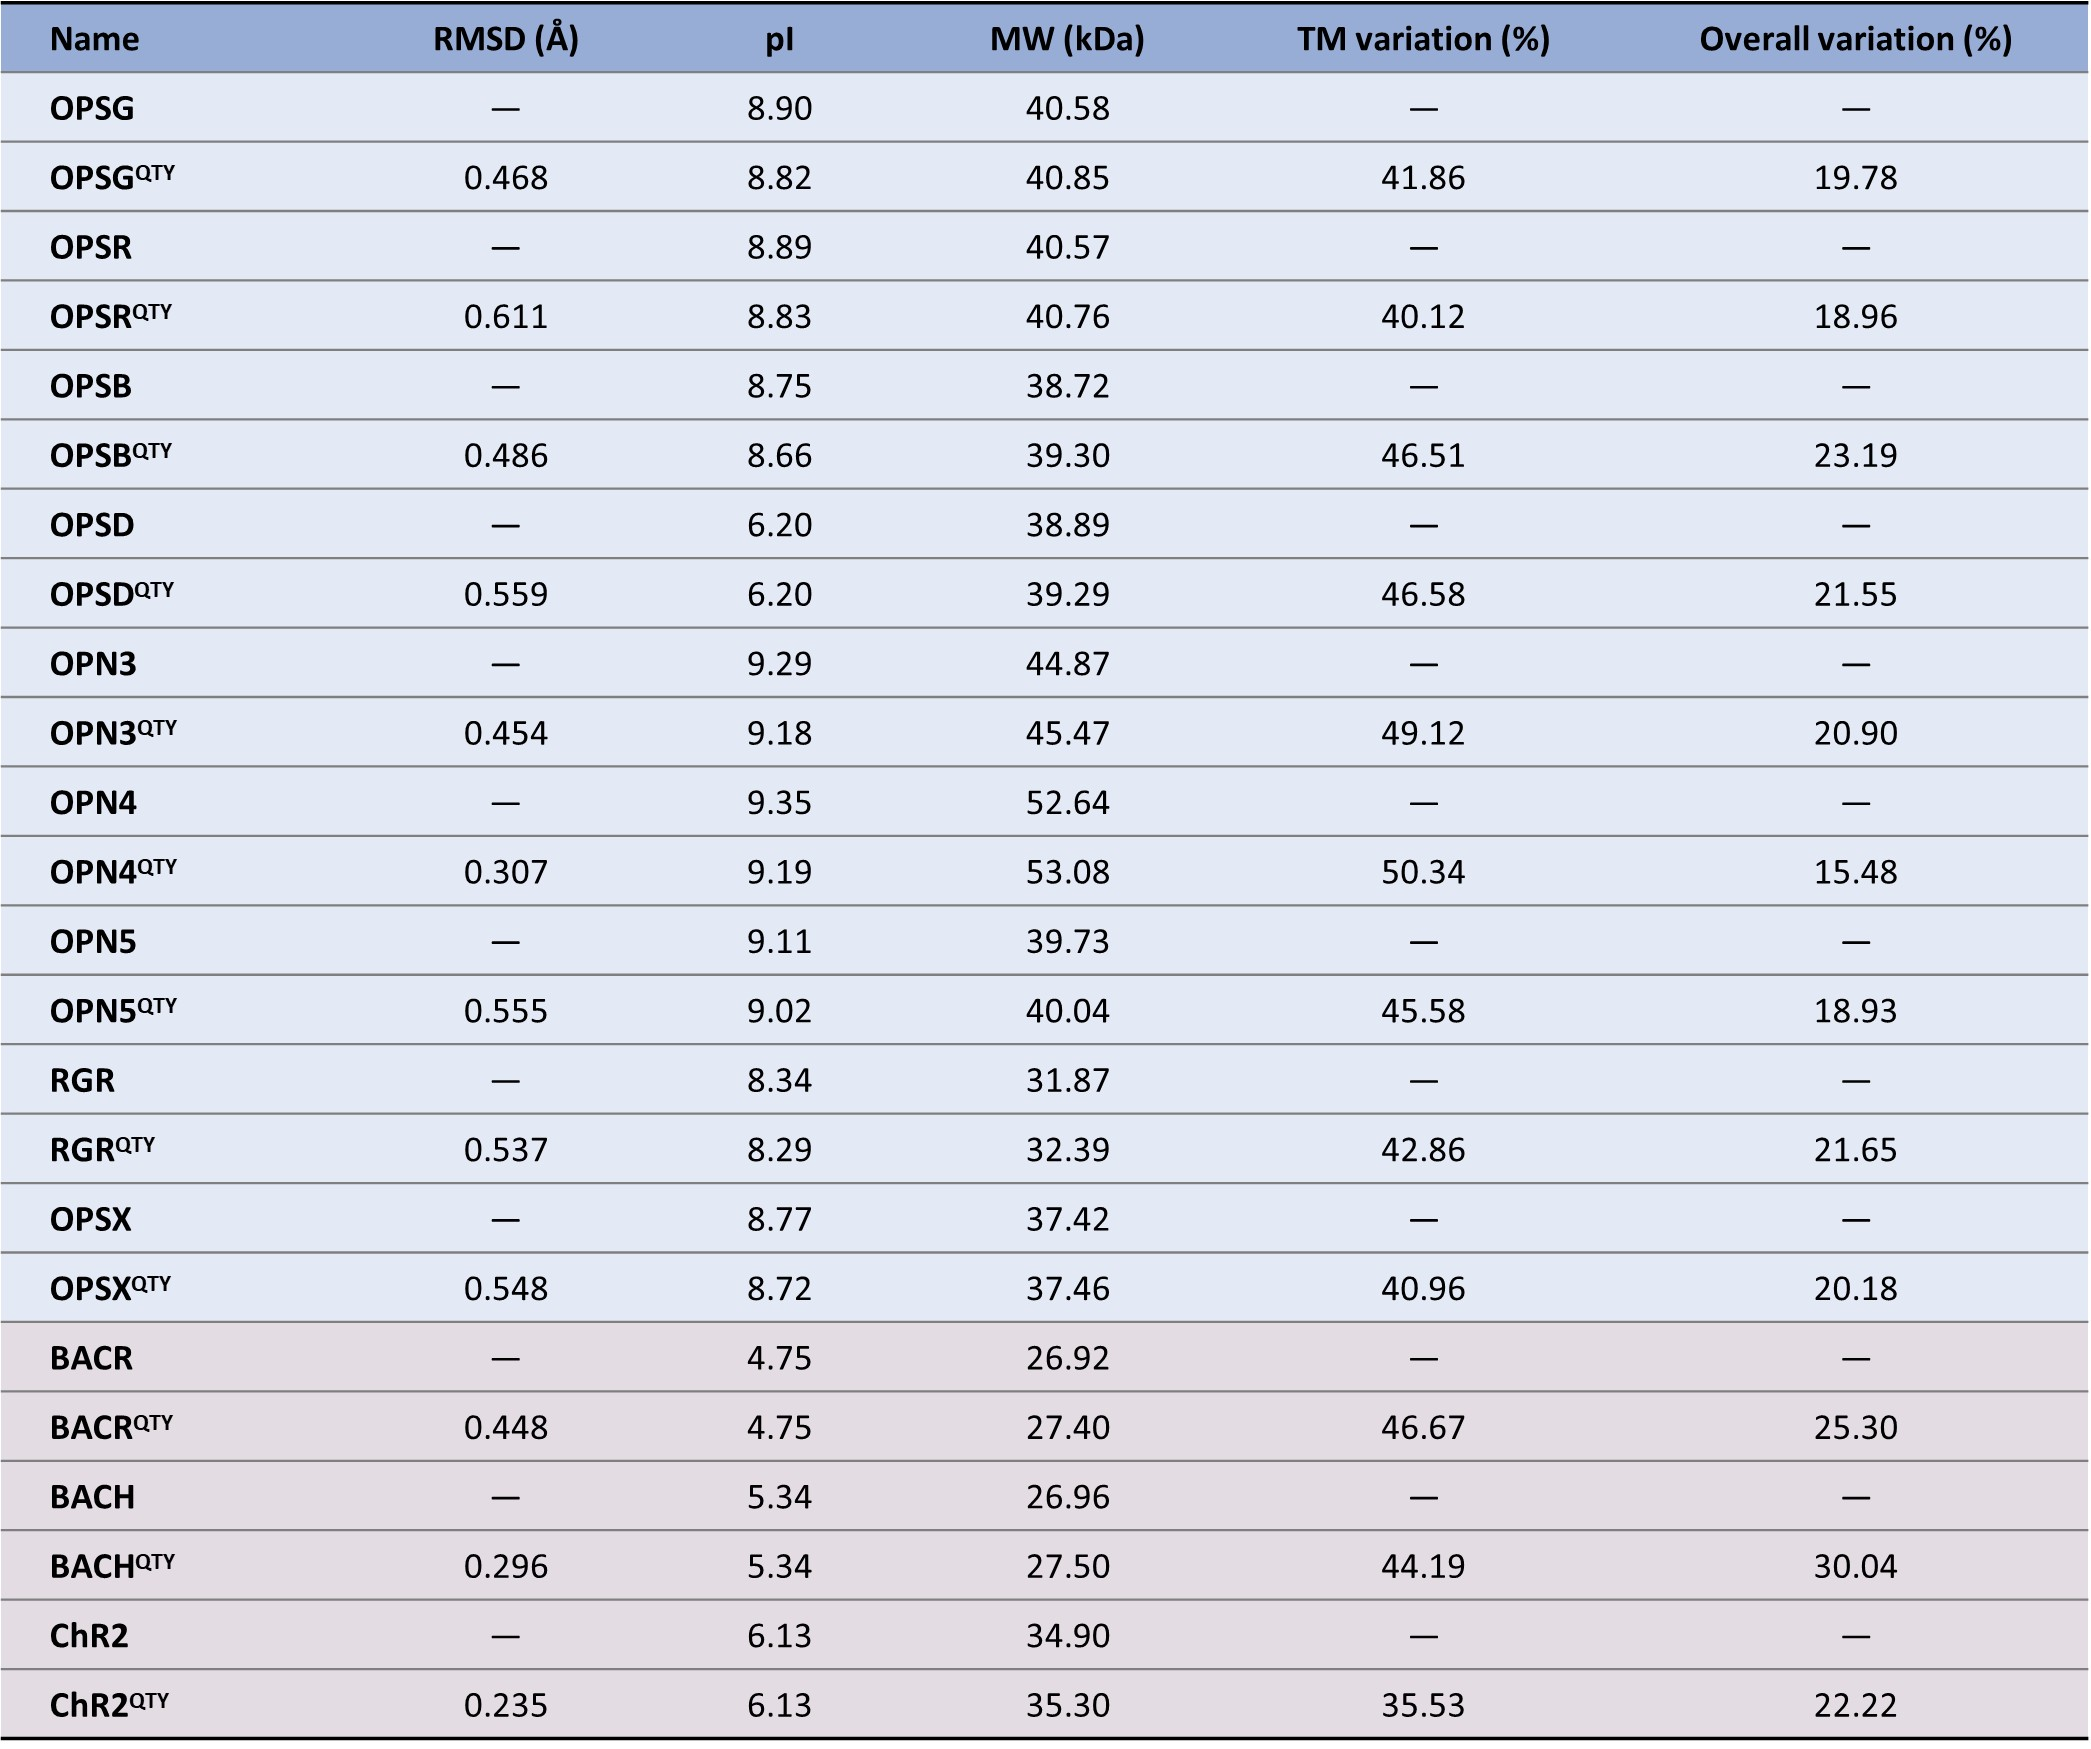
\includegraphics[width=\linewidth]{figures/characteristics.jpg}
\end{table}


\begin{figure}[h]
	\centering
	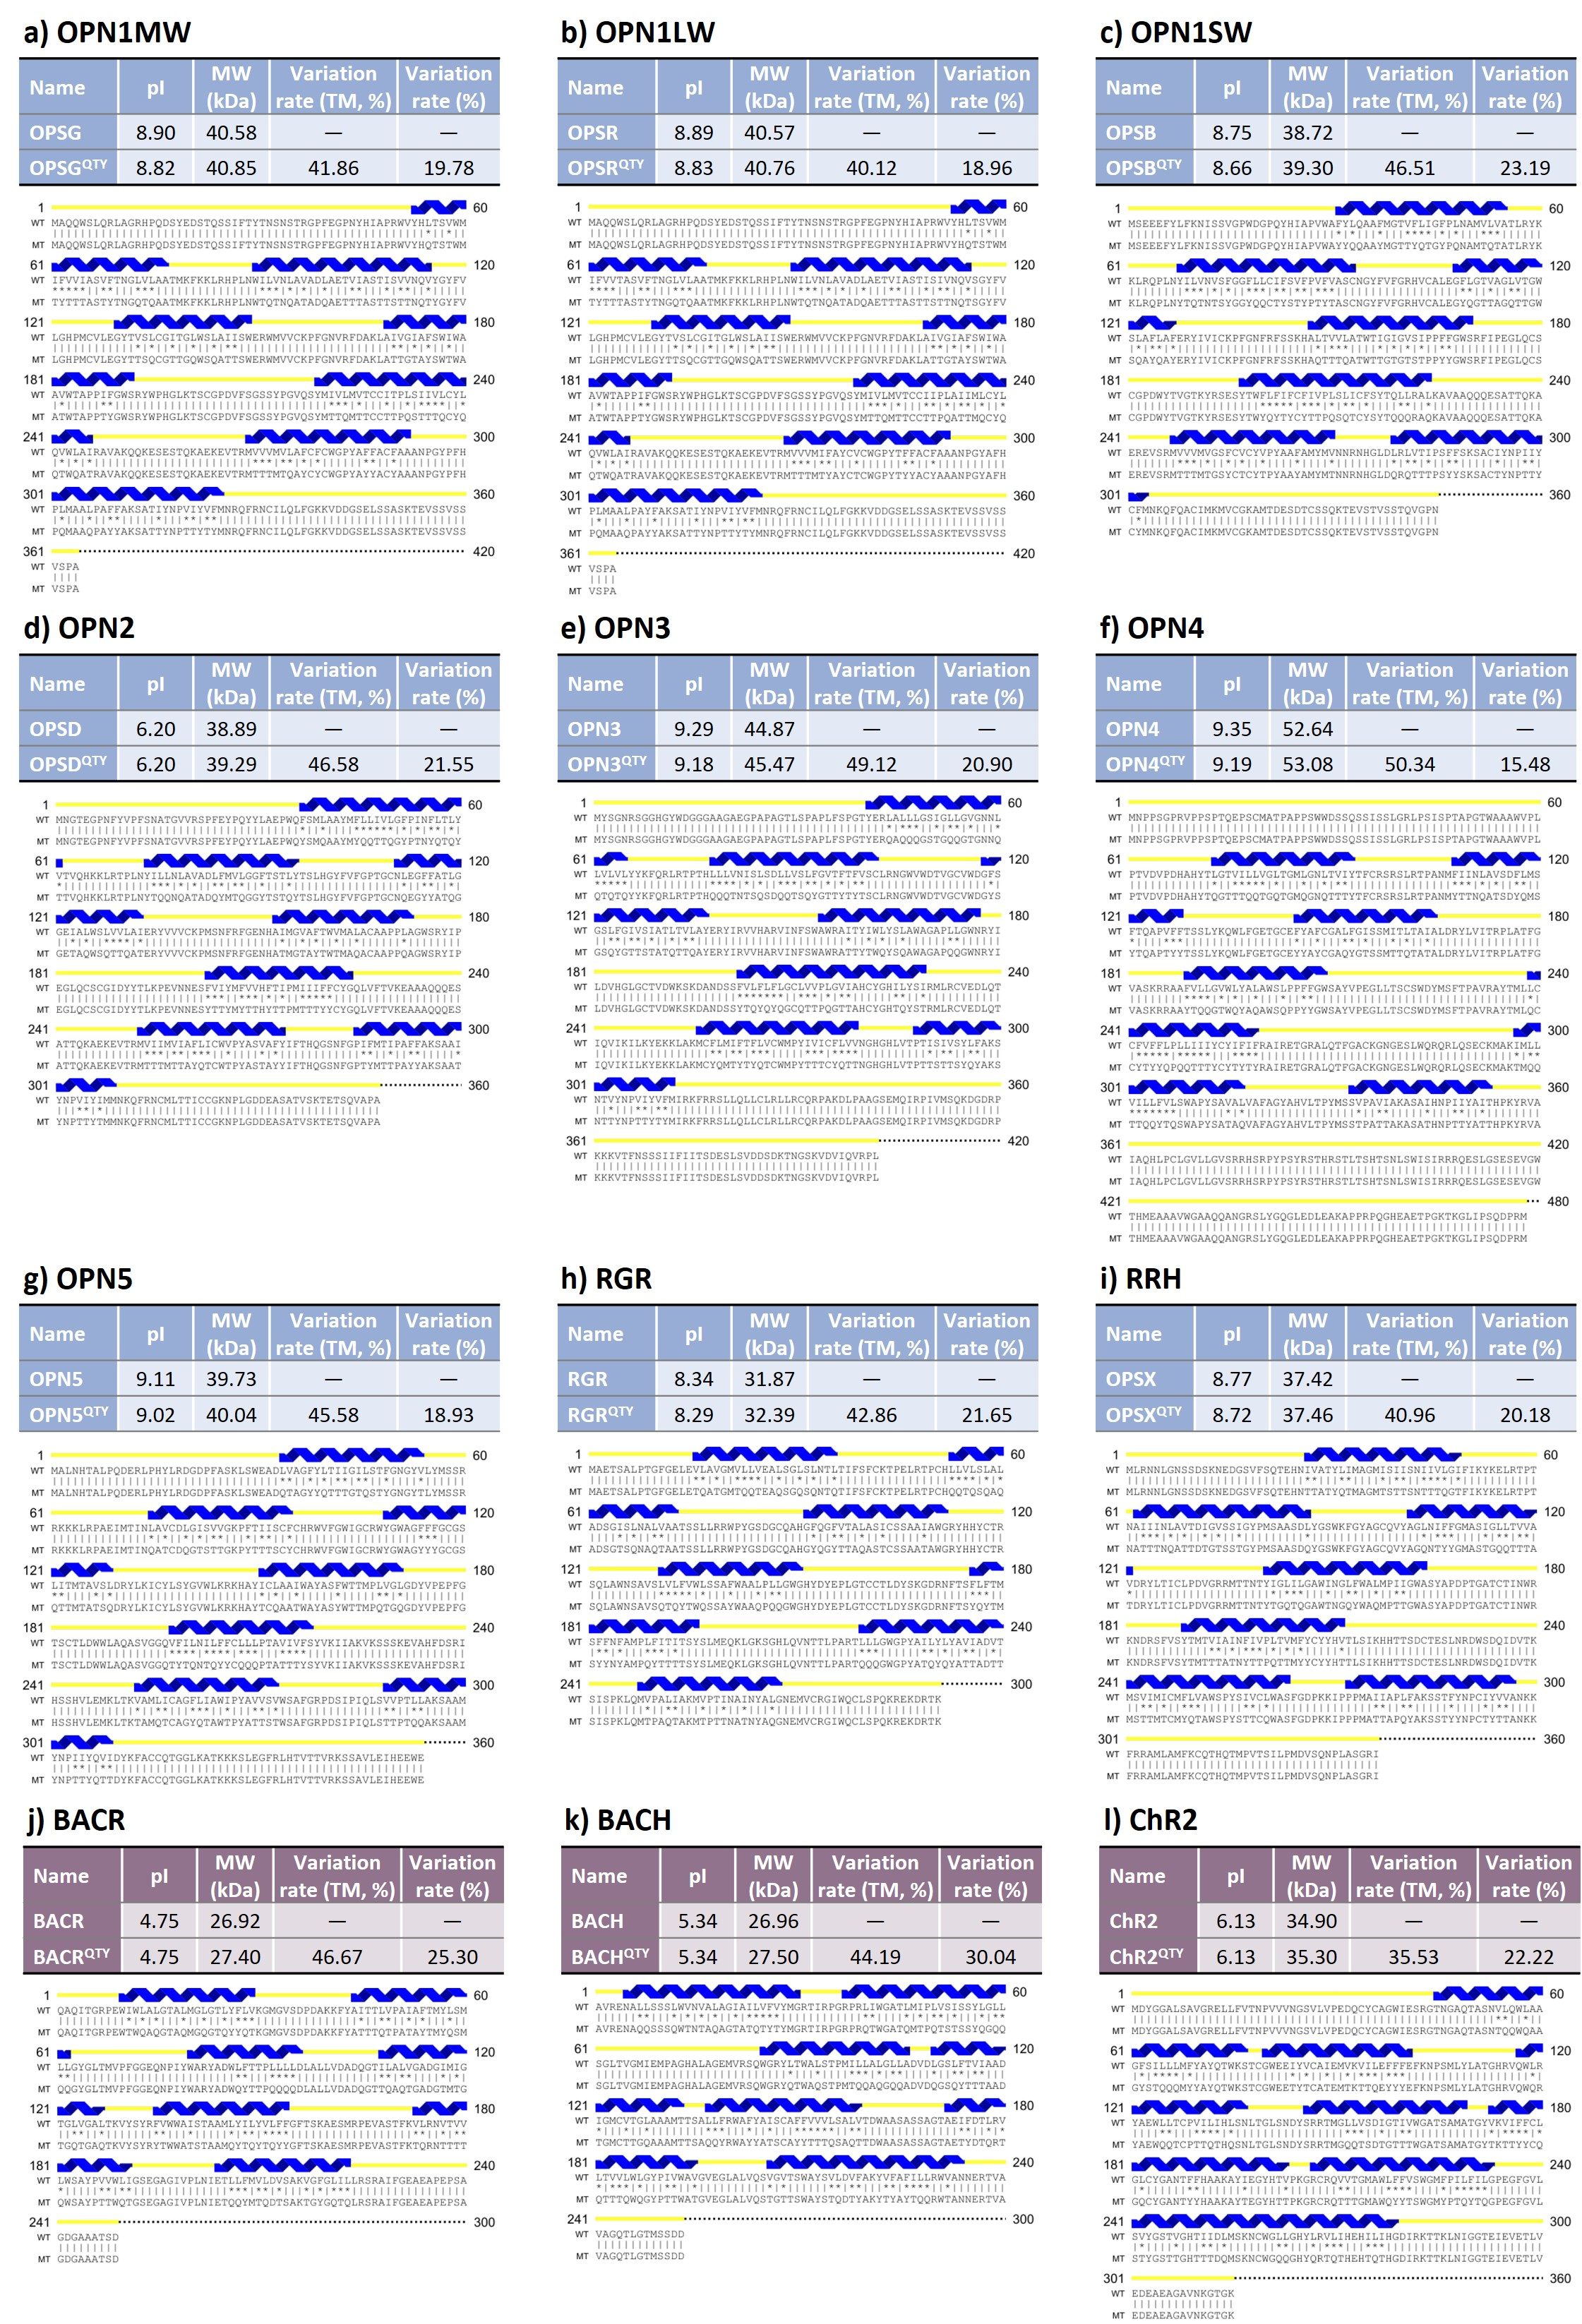
\includegraphics[width=\linewidth]{figures/sequences.jpg}
	\caption{Protein sequence alignments}
	\label{fig:sequences}
\end{figure}

\begin{figure}[h]
	\centering
	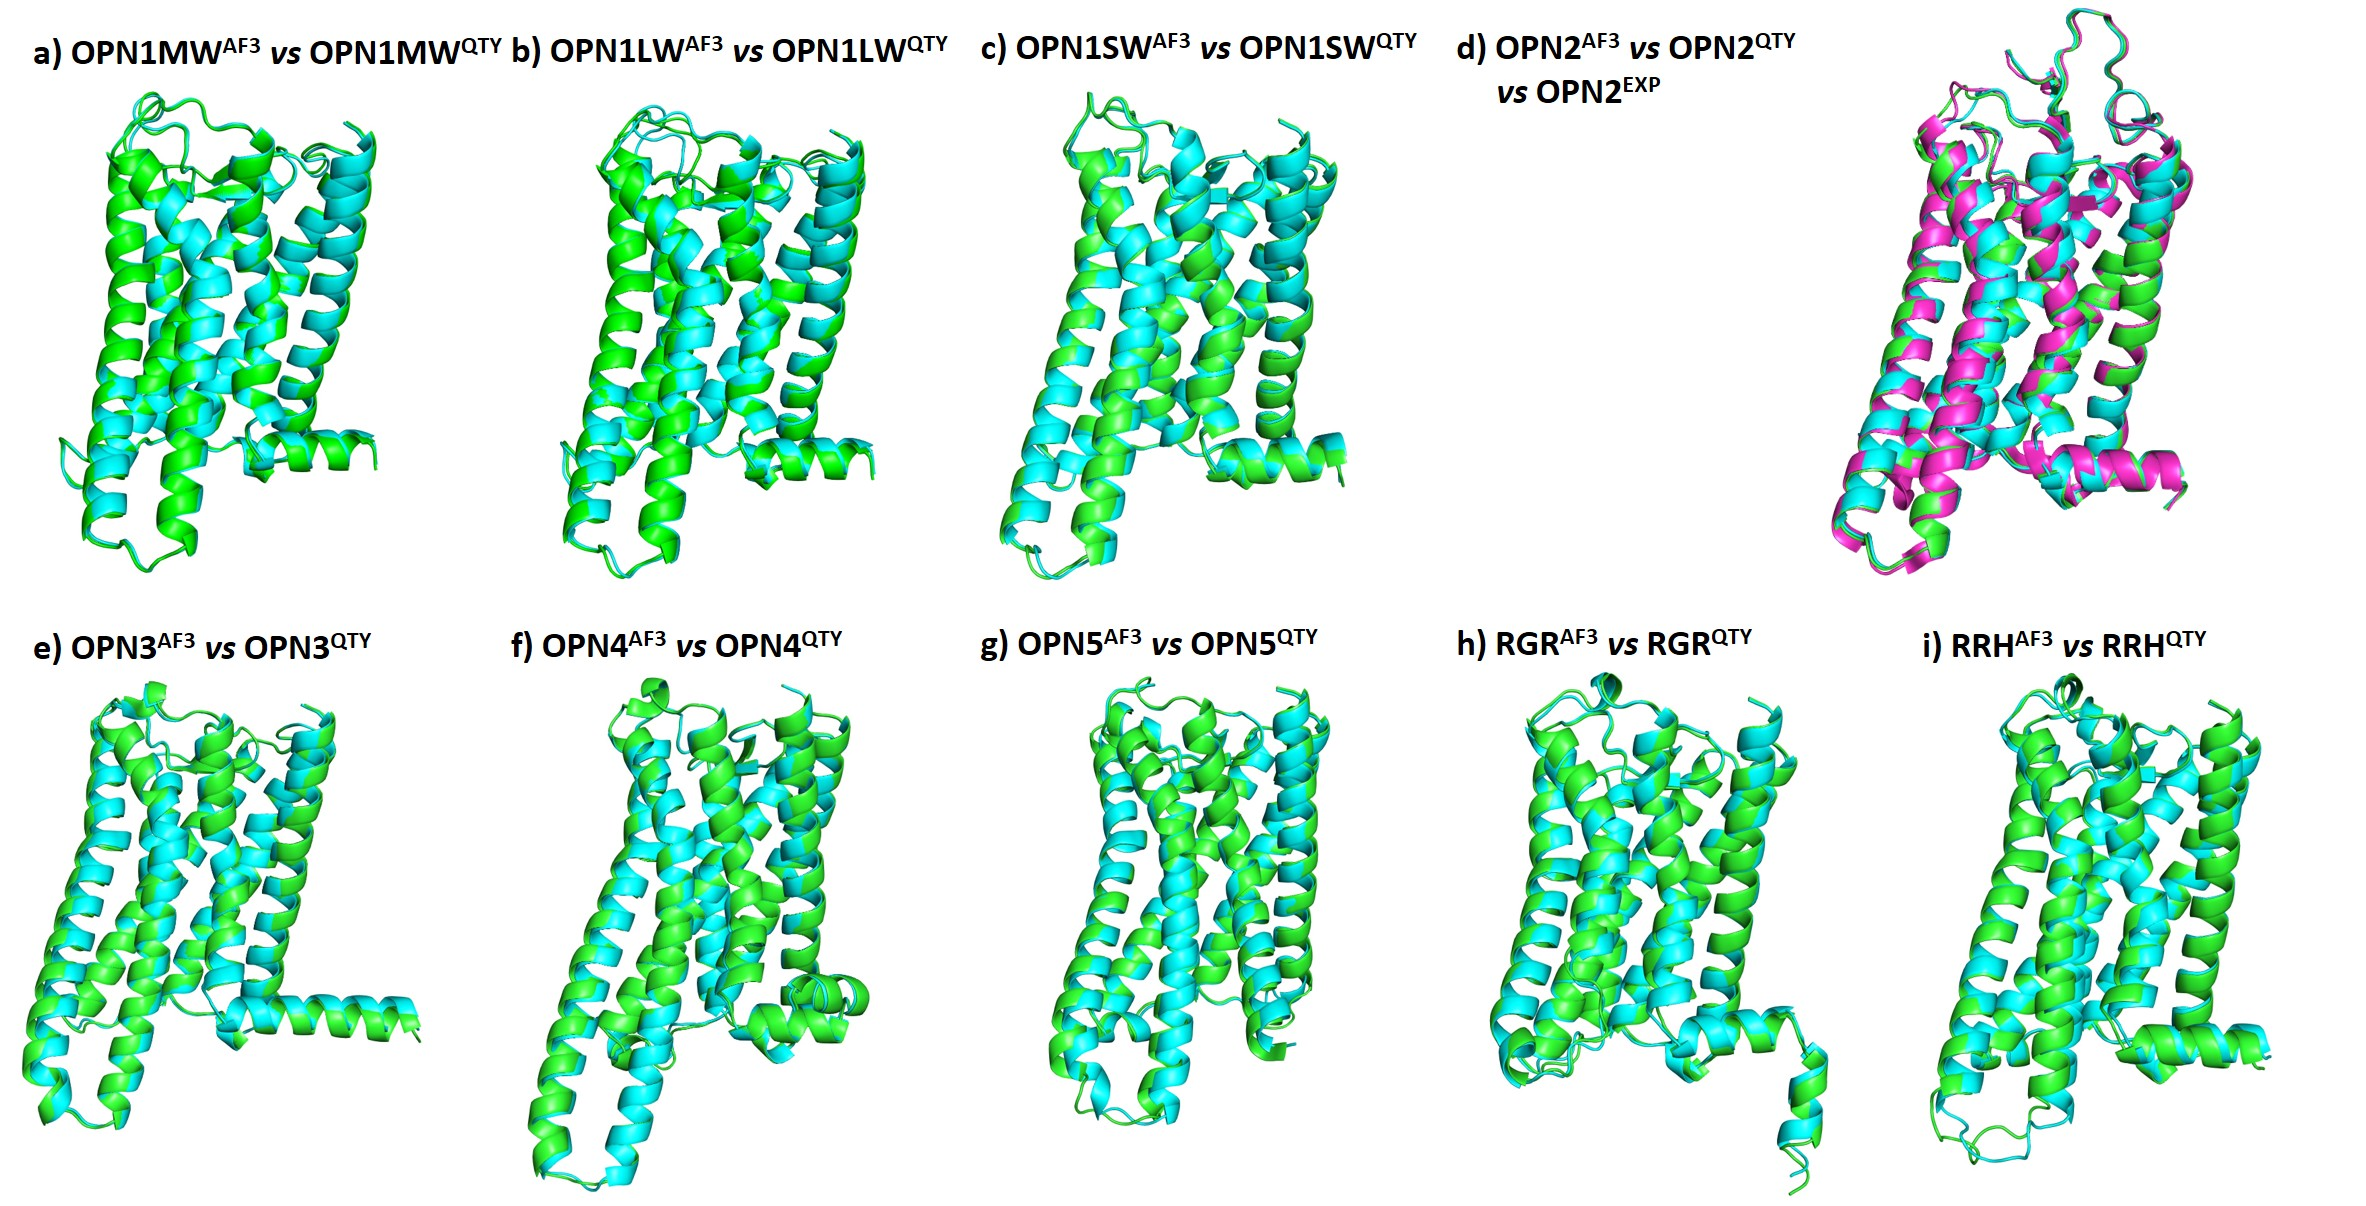
\includegraphics[width=\linewidth]{figures/superimposition-human.jpg}
	\caption{Superimposition of human retinylidene proteins}
	\label{fig:humansup}
\end{figure}

\begin{figure}[h]
	\centering
	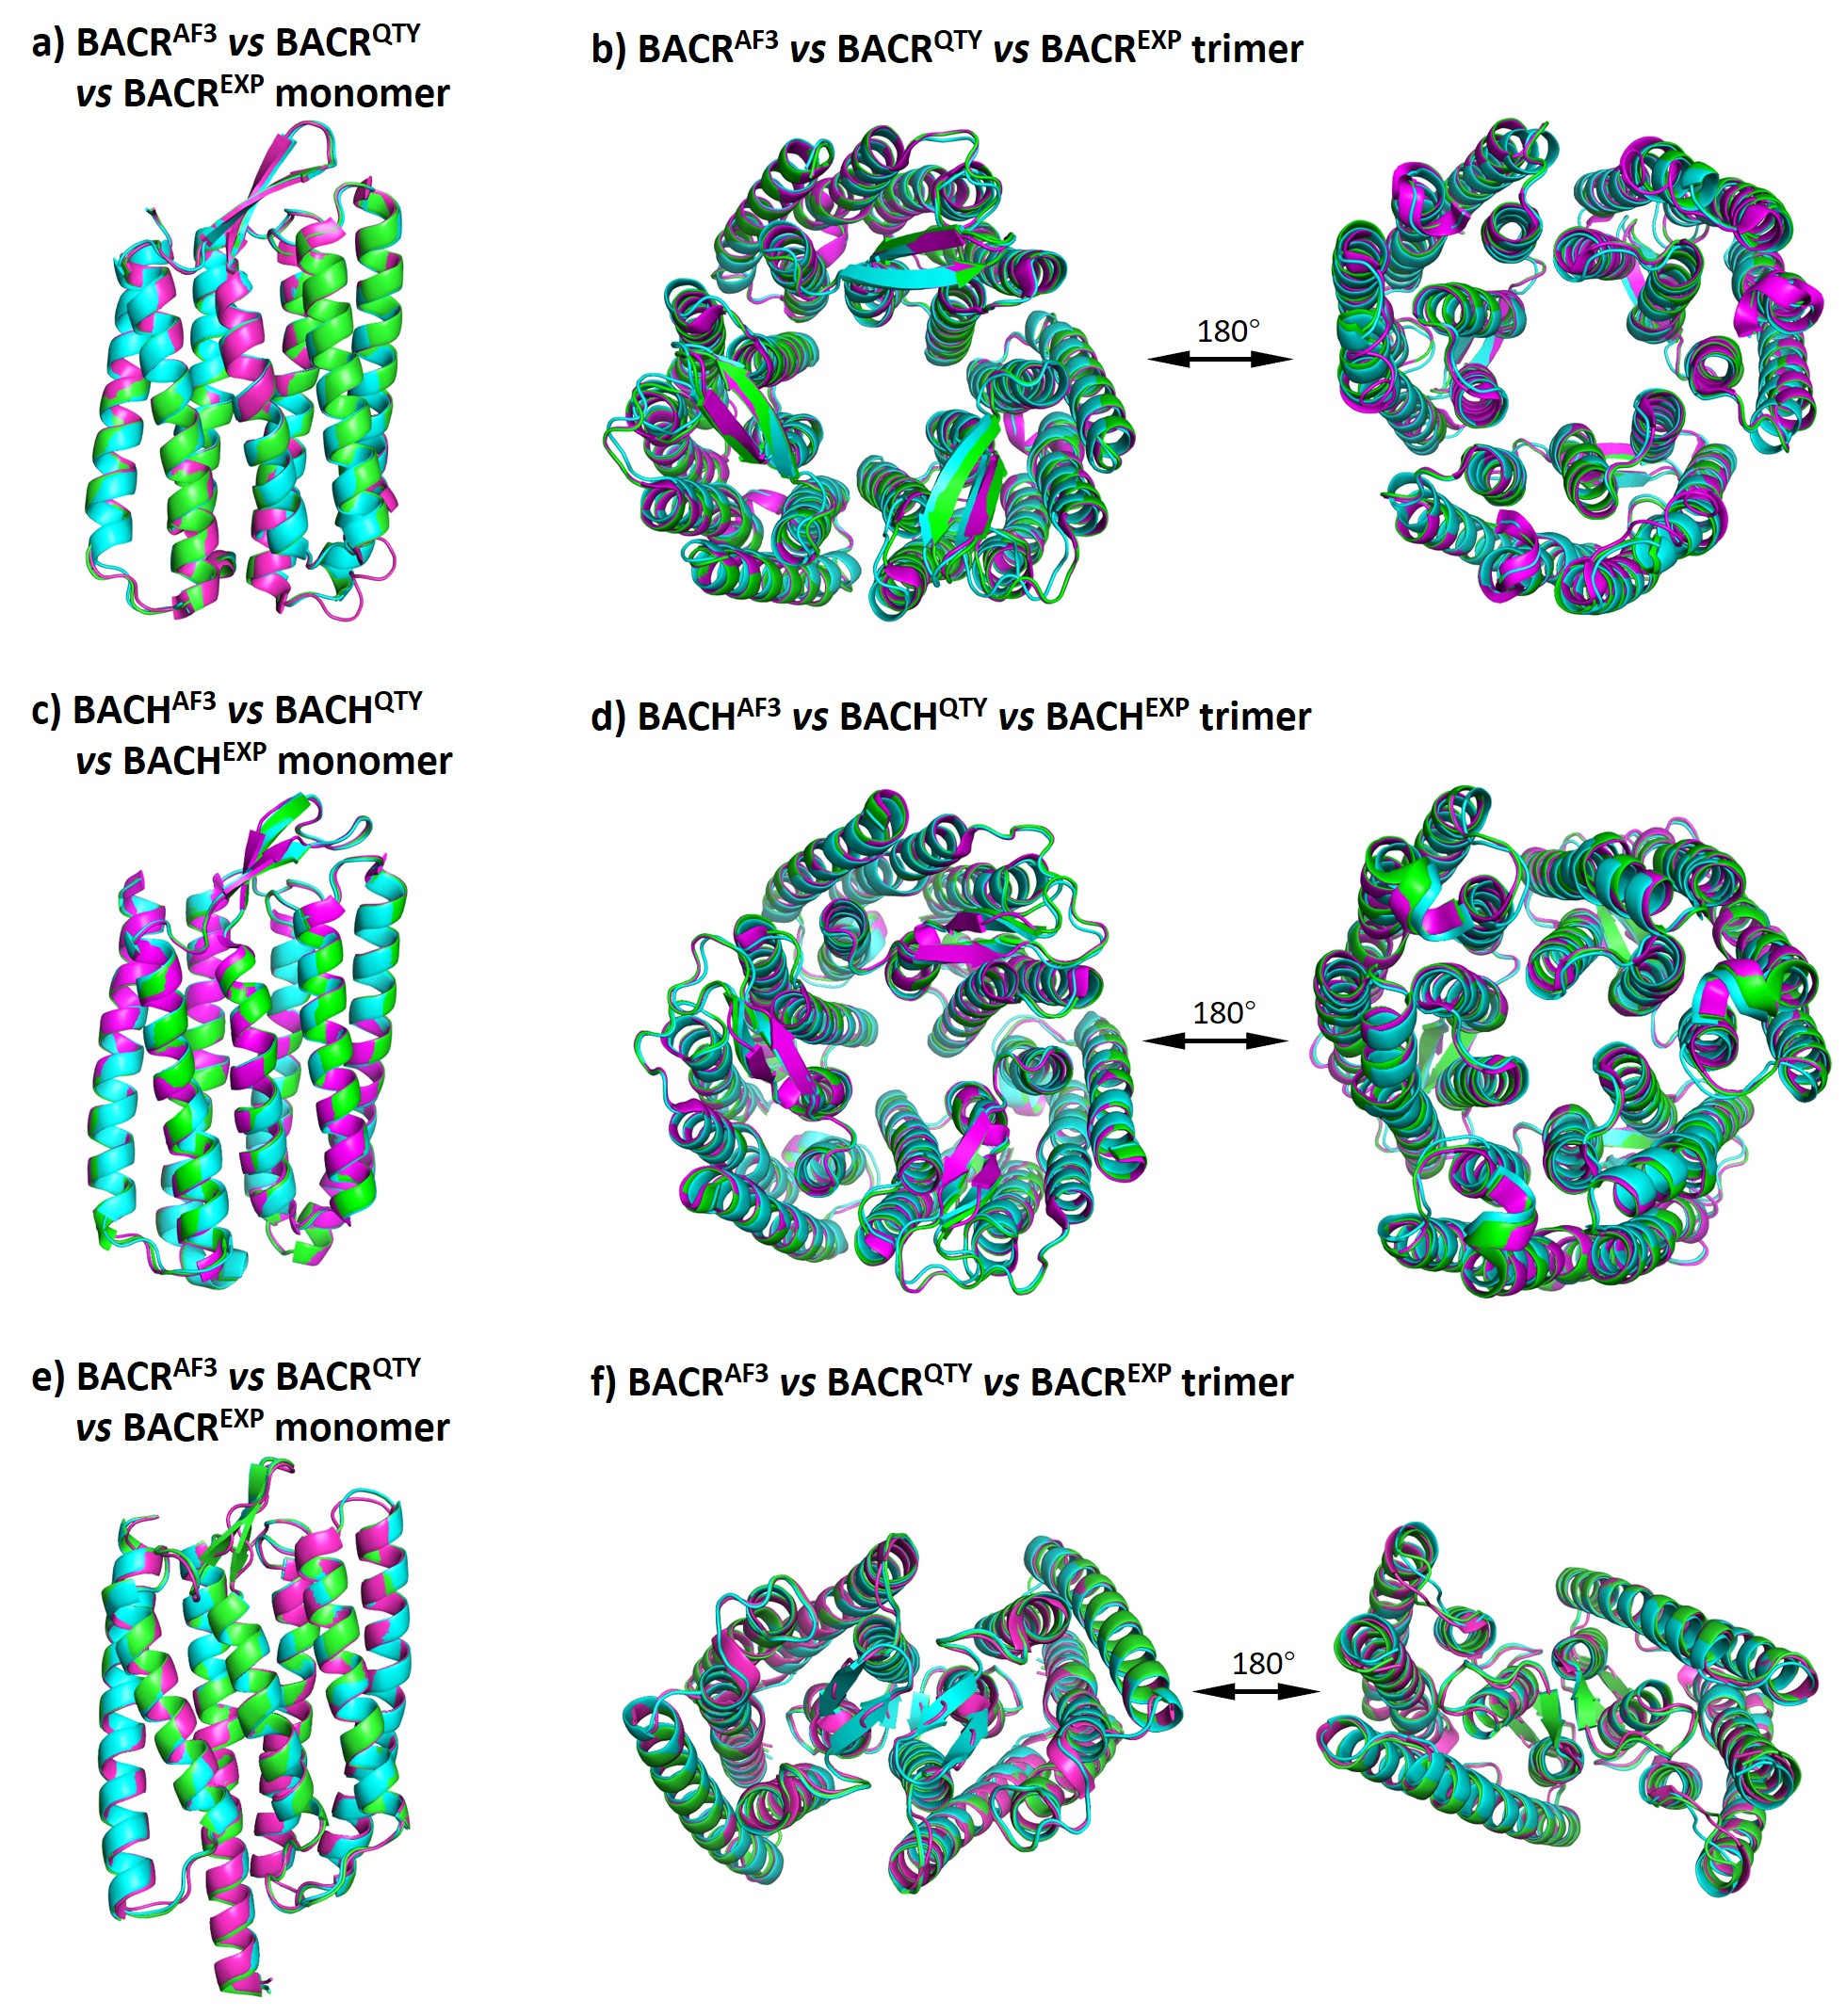
\includegraphics[width=\linewidth]{figures/superimposition-bacterial.jpg}
	\caption{Superimposition of bacterial retinylidene proteins}
	\label{fig:bacterialsup}
\end{figure}

\begin{figure}[h]
	\centering
	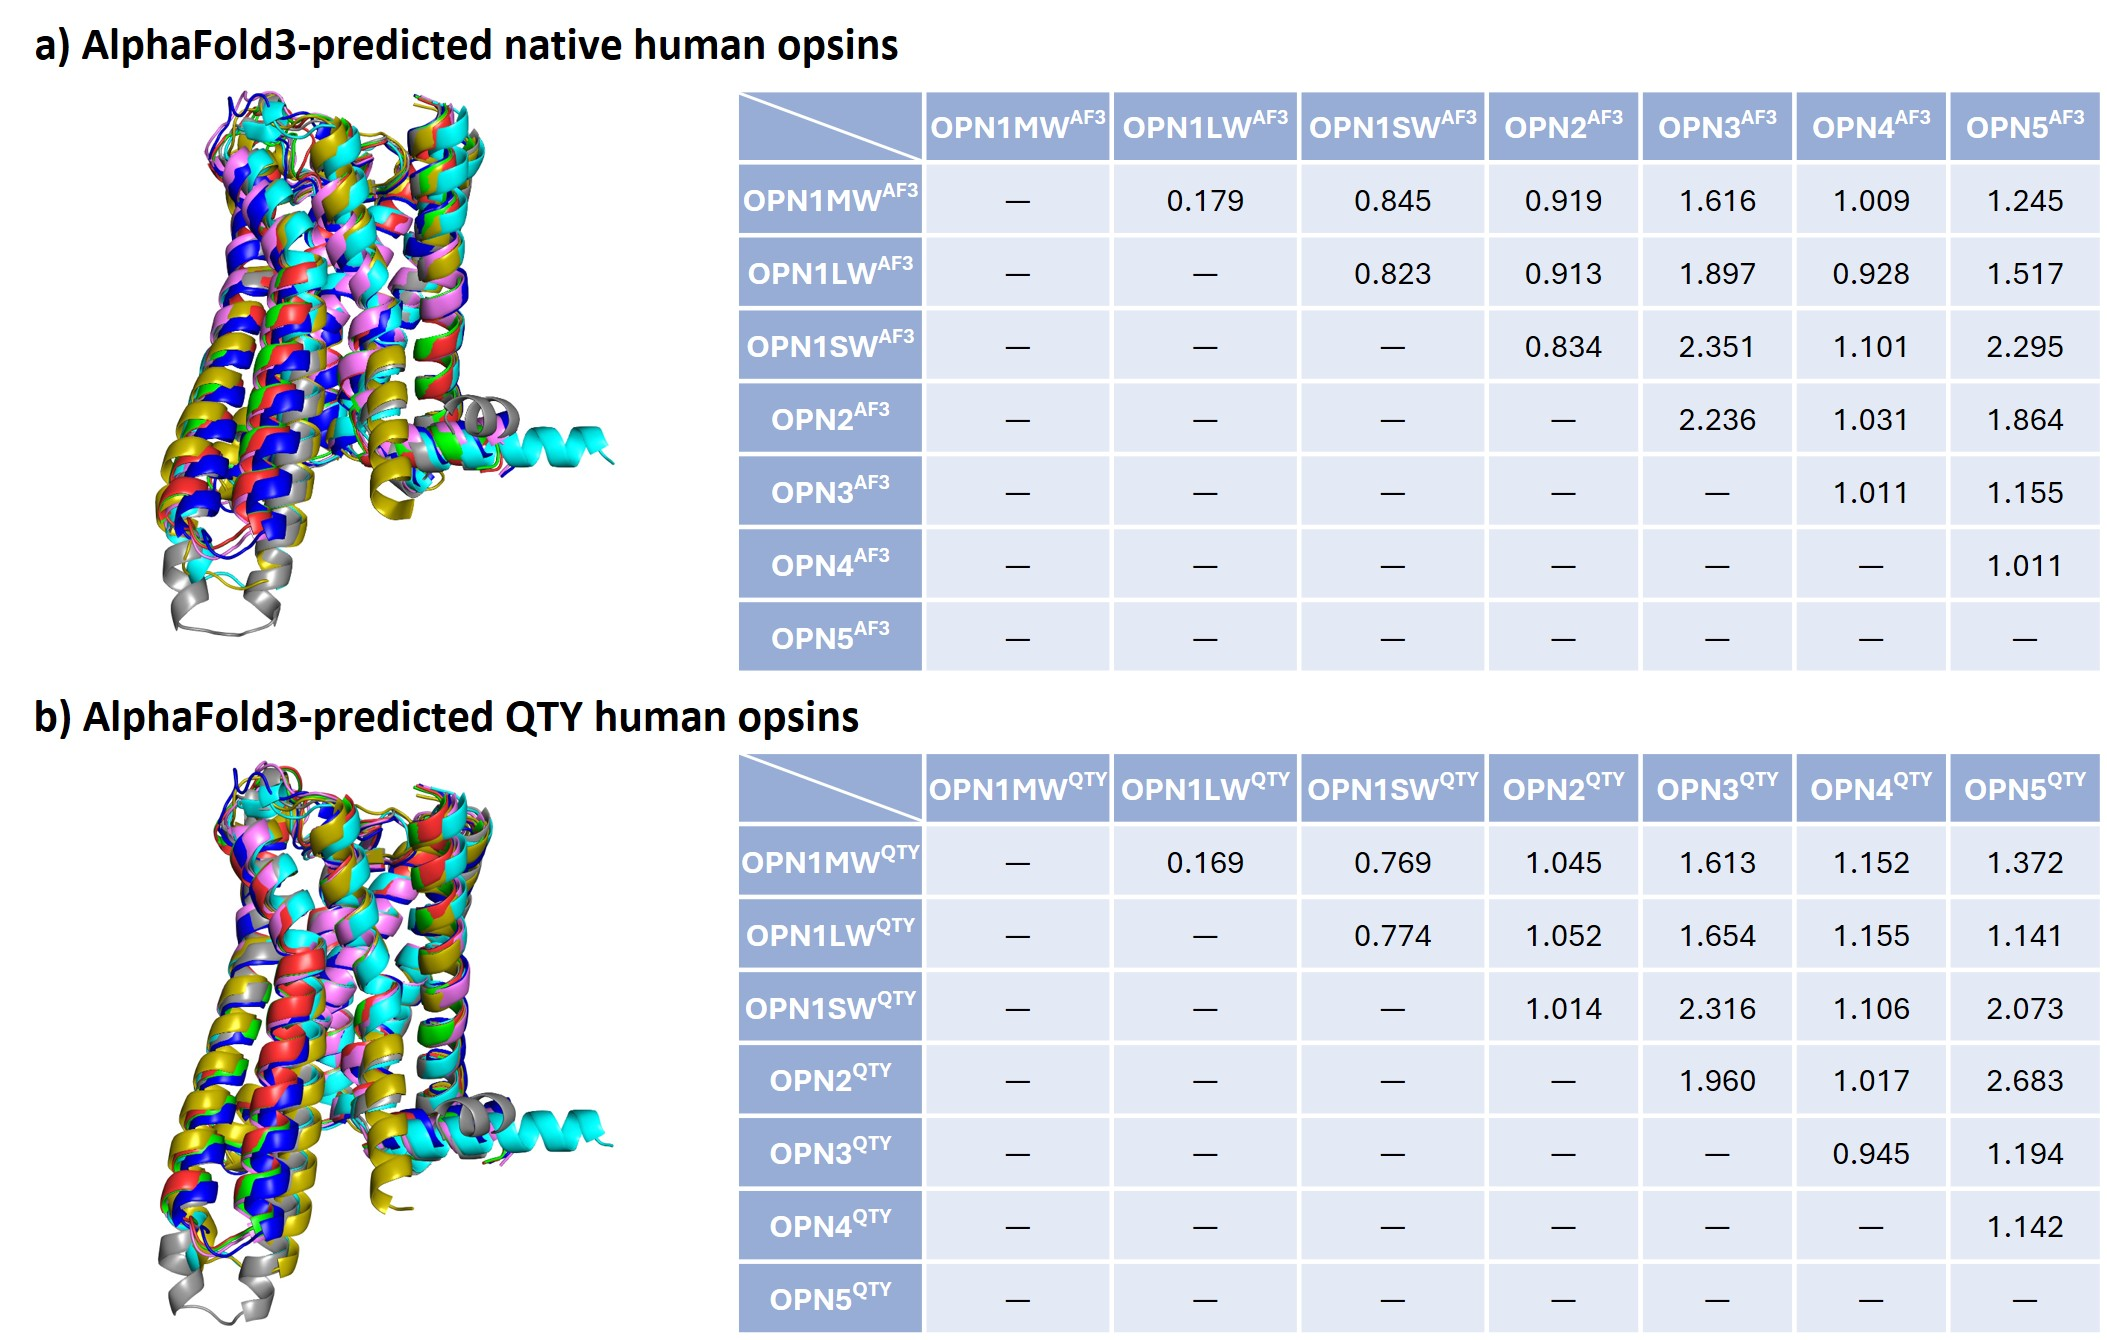
\includegraphics[width=\linewidth]{figures/pairwise.jpg}
	\caption{Pairwise comparison of human opsins}
	\label{fig:pairwise}
\end{figure}

\begin{figure}[h]
	\centering
	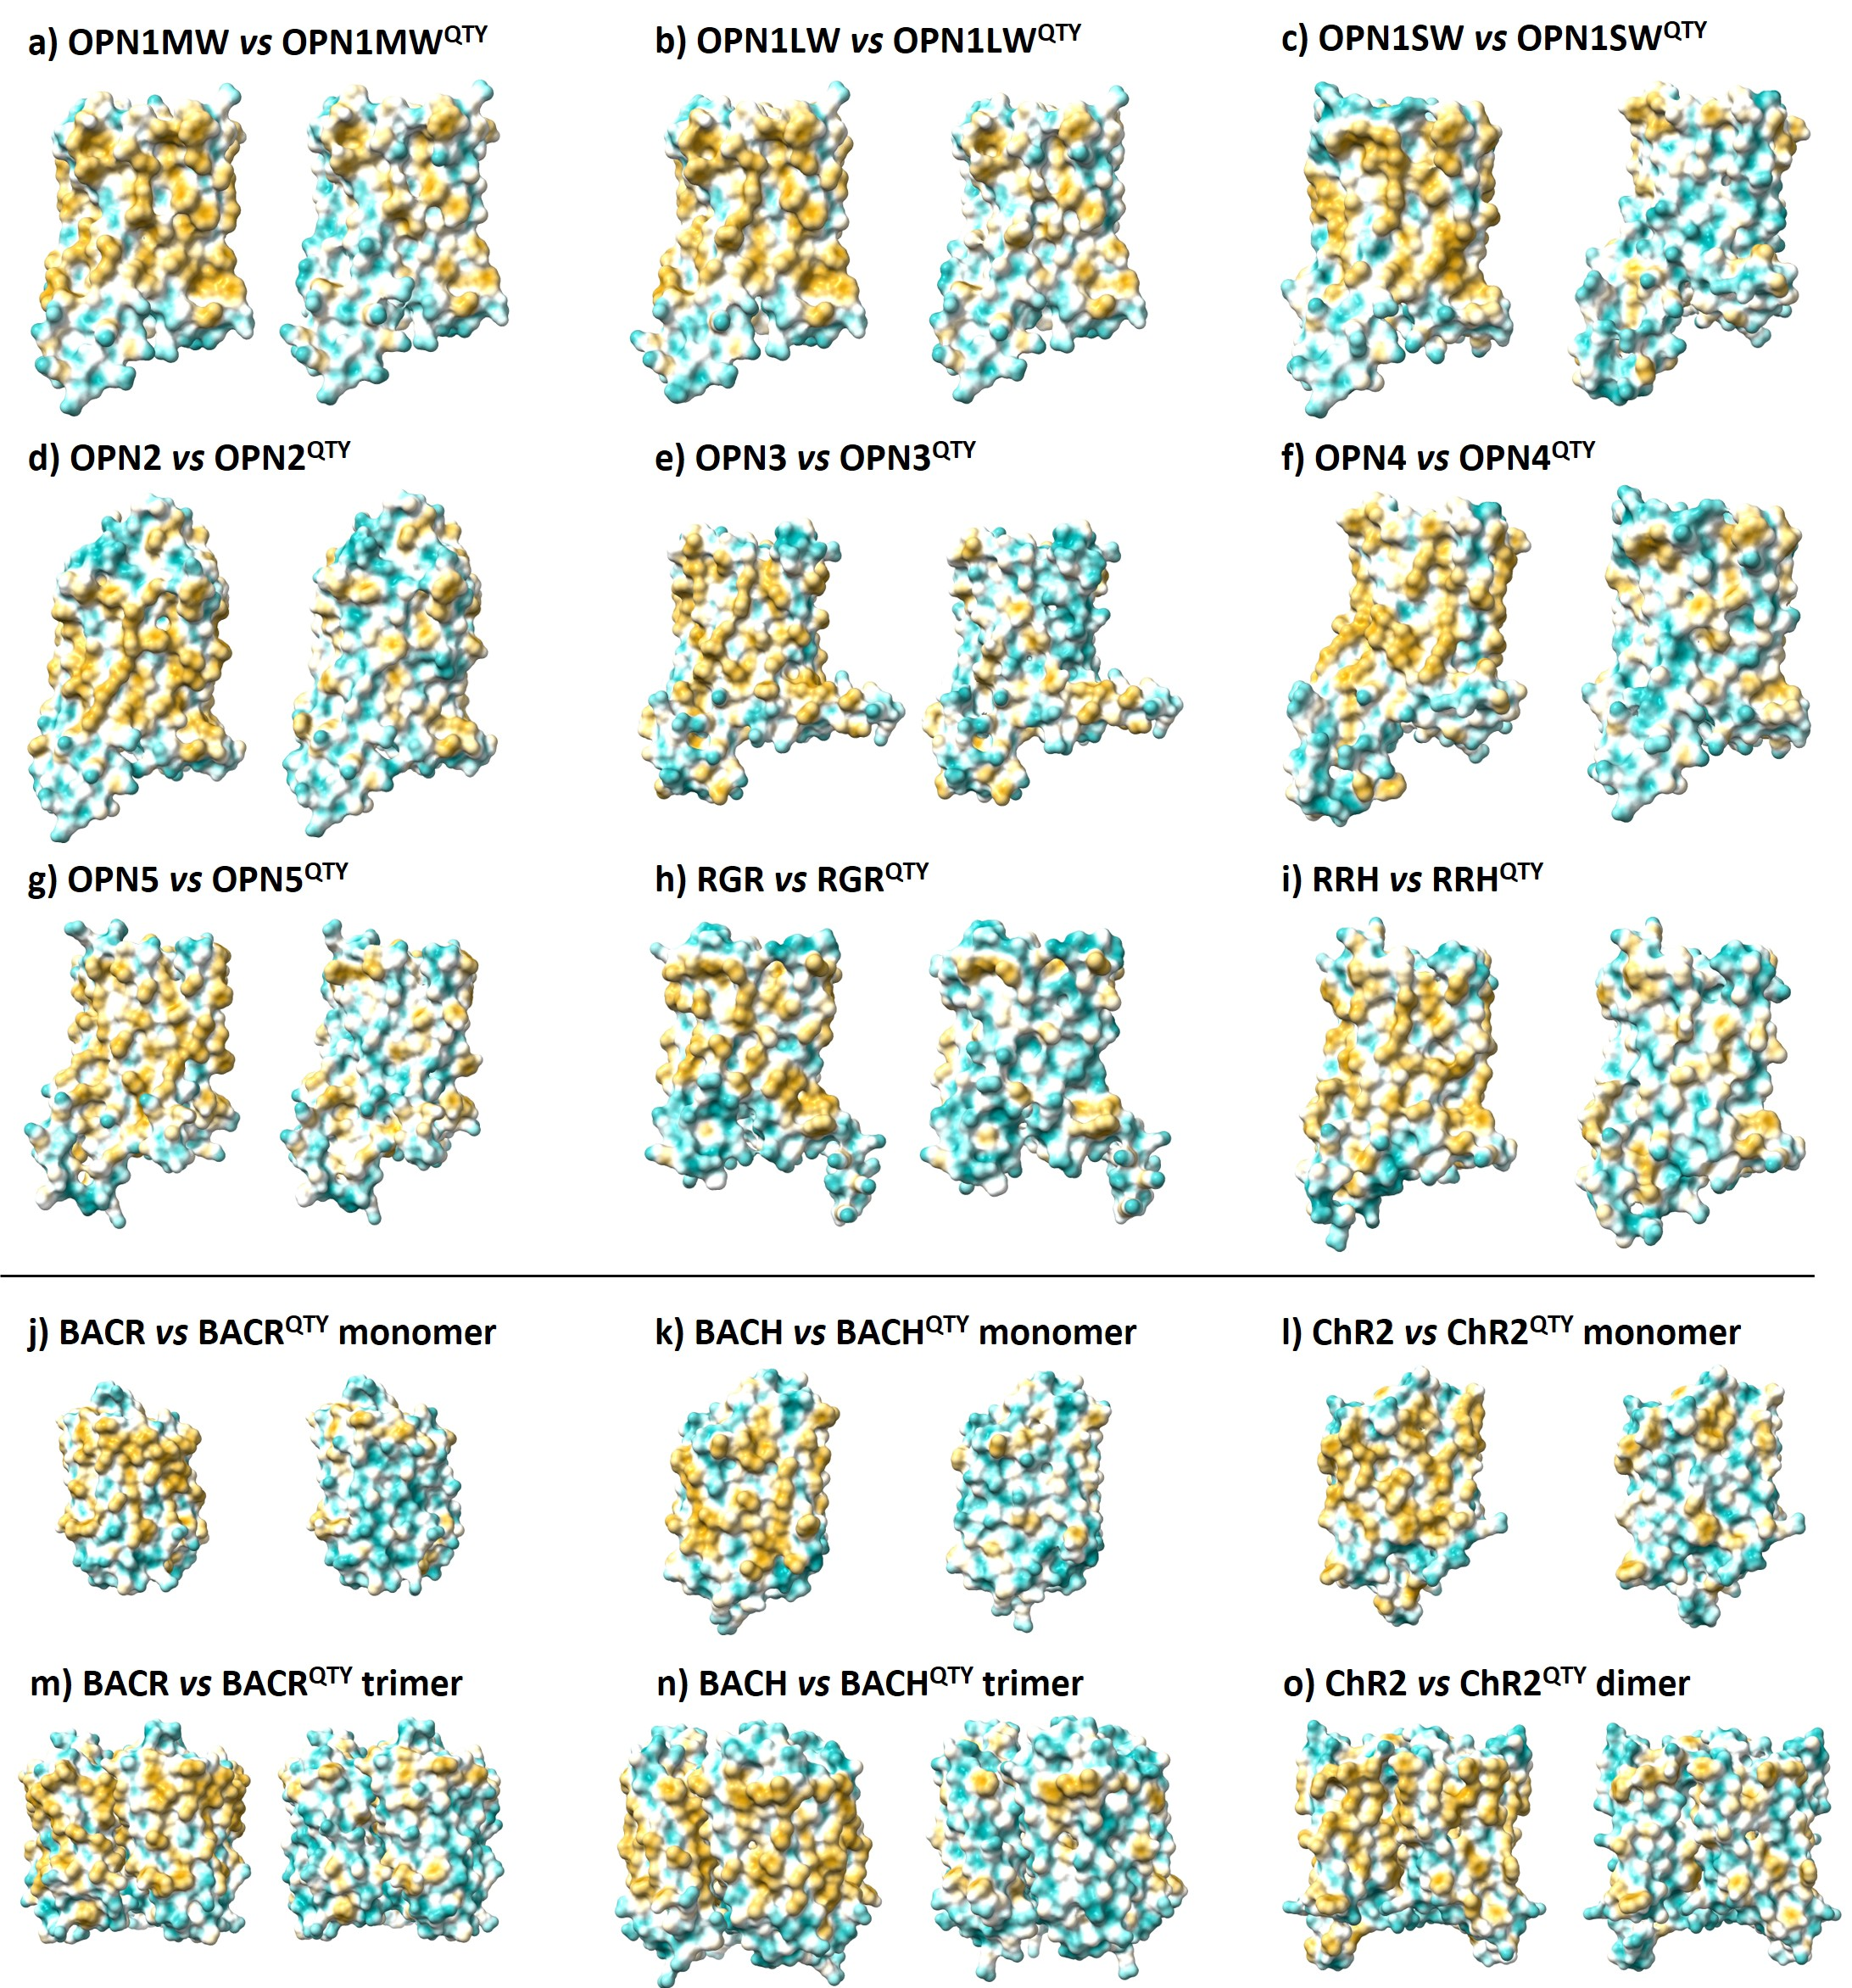
\includegraphics[width=\linewidth]{figures/hydrophobicity.jpg}
	\caption{Surface hydrophobicity}
	\label{fig:hydrophobicity}
\end{figure}

\end{document}